\documentclass{article}
\usepackage[T1]{fontenc}
\usepackage[utf8]{inputenc}

\usepackage{xspace}
\usepackage{graphicx}
\usepackage{amsmath}
\usepackage{amsfonts}
\usepackage{subfig}
\usepackage{fullpage}
\usepackage{url,paralist}
\usepackage{caption}
\usepackage{slashbox}

\author{Philip Pickering\\ \url{pgpick@gmx.at} \and Marco Eilers\\ \url{eilers.marco@googlemail.com} \and Thomas Bracht Laumann Jespersen\\ \url{ntl316@alumni.ku.dk}}
\title{Statistical Methods for Machine Learning\\ Assignment 2: Basic Learning Algorithms}
\date{}

\newcommand{\vect}[1]{\ensuremath{\boldsymbol{\mathbf{#1}}}\xspace}

%% For readability in question 1.3
\newcommand{\Target}{\vect{\mathsf{T}}}
\newcommand{\vPhi}{\vect{\Phi}}
\newcommand{\vw}{\vect{w}}
\newcommand{\Szero}{\vect{S}_0}
\newcommand{\mzero}{\vect{m}_0}
\newcommand{\target}{\vect{\mathsf{t}}}

\newcommand{\knollA}{\textsc{knollA}\xspace}
\newcommand{\knollB}{\textsc{knollB}\xspace}
\newcommand{\knollC}{\textsc{knollC}\xspace}

%% %% Uncomment these lines to get a box around all figures
%% \usepackage{float}
%% \floatstyle{boxed}
%% \restylefloat{figure}

\begin{document}
\maketitle

\section{Neural Networks}

\subsection{Neural Network implementation}

Implement a multi-layer neural network with linear output neuron and a
single hidden layer with non-linear neuron. All neurons should have
bias (offset) parameters.

To find the derivative of the activation function:
\[
\sigma(u) = \frac{|u|}{1 + |u|}
\]
we apply the quotient rule for differantiation:
\[
\frac{d}{du}\frac{f(x)}{g(x)} = \frac{g(x)f'(x) - g'(x)f(x)}{\left[g(x)\right]^2}
\]
where, in our case $f(u) = |u|$ and $g(u) = 1 + |u|$.
\begin{align}
  \frac{d}{du}\left(\frac{|u|}{1 + |u|}\right) &= \frac{(1 + |u|)\cdot 1 - (0 + 1)|u|}{(1 + |u|)^2}\\
  &= \frac{1 + |u| - |u|}{(1 + |u|)^2}\\
  &= \frac{1}{(1 + |u|)^2}
\end{align}

Implement backpropagation to compute gradient of error with respect to
the network parameters.

\subsection{Neural Network training}

Training of our neural network model starts from the file
\texttt{nntrain.m}. This file takes care of training the model and
plotting the results.

The MATLAB function \texttt{multiBatchTrain} performs a given number
of batch runs, meaning for each run we do a batch training round of
forward and backward propagations, accumulate the partial derivatives
and do the weight modification. In the training we do 500 iterations
of 50 runs for a total of 25,000
iterations. Fig.~\ref{fig:nnsolutions} plots $\frac{\sin{x}}{x}$
on the range $[-10,10]$ along with the predictions of our trained NN 
model for different learning rates and the training
data.

Fig.~\ref{fig:nnsolutions}(a)--(b) show the neural networks of
two hidden neurons. In fig.~\ref{fig:nnsolutions}(a) the result when
shortcuts are omitted and fig.~\ref{fig:nnsolutions}(b) the same model
trained using shortcuts.

In fig.~\ref{fig:nnsolutions}(c)--(b) is shown neural networks of 20
hidden neurons, where fig.~\ref{fig:nnsolutions}(c) is without
shortcuts and fig.~\ref{fig:nnsolutions}(d) is with.

We found it instructive to include the models trained with and without
shortcuts, because in both cases the model using shortcuts performs
better on the same learning time independently of the learning rate.

It is also clear that the highest learning rate possible (which didn't
produce numerical overflows), gave better solutions on the same
learning time.

\begin{figure}[!h]
  \centering
  \subfloat[\hfill]{\includegraphics[width=.5\textwidth]{solution2ns.eps}}
  \subfloat[\hfill]{\includegraphics[width=.5\textwidth]{solution2.eps}}

  \subfloat[\hfill]{\includegraphics[width=.5\textwidth]{solution20ns.eps}}
  \subfloat[\hfill]{\includegraphics[width=.5\textwidth]{solution20.eps}}
  \caption{Neural networks for 2 and 20 hidden neurons.}
  \label{fig:nnsolutions}
\end{figure}

Fig.~\ref{fig:nnerrors} shows the error trajectories for our different
neural networks. A learning epoch on the $x$-axis corresponds to 50
iterations of batch training, meaning when $x = 100$, a total of 5000
iterations have been performed.

Interestingly, when shortcuts are omitted, the error rate decreases
much faster than is the case when shortcuts are in use. One argument
for why this is, could be that not using shortcuts leads to a simpler
model that is faster to train (but obviously less flexible as
demonstrated by fig.~\ref{fig:nnsolutions}).

\begin{figure}[!h]
  \centering
  \subfloat{\includegraphics[width=.5\textwidth]{errors2ns.eps}}
  \subfloat{\includegraphics[width=.5\textwidth]{errors2.eps}}

  \subfloat{\includegraphics[width=.5\textwidth]{errors20ns.eps}}
  \subfloat{\includegraphics[width=.5\textwidth]{errors20.eps}}
  \caption{Error trajectories for the different NN models}
  \label{fig:nnerrors}
\end{figure}


\newpage
\section{Support Vector Machines}

For this part of the assignment we chose to use the LIBSVM library.

\subsection{Model Selection}
The LIBSVM manual recommends to try an exponentially growing sequence of numbers for $\gamma$. Since the default value LIBSVM uses is $1/n$ and our $n$ equals (multiples of) 100, 0.001 should likely be included in this sequence. We therefore did the grid search using the following values of $\gamma: \{ 0.0001, 0.001, 0.01, 0.1, 1, 10, 100 \}$. 

LIBSVM has built-in functionality to perform $n$-fold cross validation
given a command line option. To perform model selection we iterate
through all combinations of $C$ and $\gamma$ and call a function
called \texttt{crossval}, which invokes LIBSVM to perform a 5-fold
cross validation on the current values of $C$ and $\gamma$. When
performing $n$-fold cross validation, LIBSVM returns the accuracy,
which we  use to keep track of the configuration that gives the
highest accuracy.

Applied to the testdata, this gives the results in tables ~\ref{tab:crossval100} to ~\ref{tab:crossval400}. The resulting optimal parameter configurations are shown in table ~\ref{tab:svmoptimal}.

\begin{table}[!h]
  \centering
  \begin{tabular}{l | c | c | c | c | c | c}
    \backslashbox{$\gamma$}{$C$} & $0.1$ & $1$ & $10$ & $100$ & $1000$ & $10000$\\\hline
    $0.0001$ & 55\% & 55\% & 55\% & 55\% & 55\% & 55\% \\
    $0.001$ & 55\% & 55\% & 55\% & 55\% & 55\% & 65\% \\
    $0.01$ & 55\% & 55\% & 56\% & 57\% & 65\% & 98\% \\
    $0.1$ & 60\% & 60\% & 59\% & 63\% & 98\% & 95\% \\
    $1$ & 57\% & 58\% & 59\% & 92\% & 97\% & 94\% \\
    $10$ & 51\% & 54\% & 67\% & 88\% & 92\% & 91\% \\
    $100$ & 52\% & 47\% & 76\% & 76\% & 77\% & 77\% \\
  \end{tabular}
  \caption{Table of all results for model selection using grid-search
    for \texttt{knollC-train100}.}
  \label{tab:crossval100}
\end{table}

\begin{table}[!h]
  \centering
  \begin{tabular}{l | c | c | c | c | c | c}
    \backslashbox{$\gamma$}{$C$} & $0.1$ & $1$ & $10$ & $100$ & $1000$ & $10000$\\\hline
    $0.0001$ & 49.5\% & 49.5\% & 49.5\% & 49.5\% & 50.5\% & 53\% \\
    $0.001$ & 49.5\% & 49.5\% & 49.5\% & 59.5\% & 52.5\% & 78.5\% \\
    $0.01$ & 50\% & 50\% & 51\% & 51\% & 75.5\% & 97.5\% \\
    $0.1$ & 48\% & 49.5\% & 49\% & 76\% & 97.5\% & 96\% \\
    $1$ & 50\% & 51\% & 59\% & 96\% & 97\% & 96.5\% \\
    $10$ & 54\% & 52\% & 86.5\% & 96\% & 93\% & 94.5\% \\
    $100$ & 57\% & 62\% & 90.5\% & 91.5\% & 91\% & 91\% \\
  \end{tabular}
  \caption{Table of all results for model selection using grid-search
    for \texttt{knollC-train200}.}
  \label{tab:crossval200}
\end{table}

\begin{table}[!h]
  \centering
  \begin{tabular}{l | c | c | c | c | c | c}
    \backslashbox{$\gamma$}{$C$} & $0.1$ & $1$ & $10$ & $100$ & $1000$ & $10000$\\\hline
    $0.0001$ & 56\% & 56\% & 56\% & 56\% & 56.25\% & 60\% \\
    $0.001$ & 55.75\% & 55.75\% & 55.75\% & 56\% & 56.5\% & 96.75\% \\
    $0.01$ & 53.25\% & 53.25\% & 53.5\% & 57\% & 96.5\% & 97.5\% \\
    $0.1$ & 52.75\% & 52\% & 50.5\% & 95.75\% & 97.5\% & 97.5\% \\
    $1$ & 54.25\% & 55\% & 81.75\% & 97.5\% & 97\% & 96.75\% \\
    $10$ & 55.25\% & 61\% & 94\% & 96.5\% & 96\% & 95.75\% \\
    $100$ & 59.5\% & 81.5\% & 92\% & 93\% & 92.25\% & 90.5\% \\
  \end{tabular}
  \caption{Table of all results for model selection using grid-search
    for \texttt{knollC-train400}.}
  \label{tab:crossval400}
\end{table}

%% Result: best parameters are:
%% C: 1000, gamma: 0.100000 Cross Validation Accuracy = 98%
%% C: 1000, gamma: 0.100000 Cross Validation Accuracy = 97.5%
%% C: 100, gamma: 1.000000 Cross Validation Accuracy = 97.5%
\begin{table}[!h]
  \centering
  \begin{tabular}{l | c | c | c }
    \hfill & $C$ & $\gamma$ & Acc.\\\hline
    \texttt{knollC-train100} & 1000 & 0.1 & 98\%\\
    \texttt{knollC-train200} & 1000 & 0.1 & 97.5\%\\
    \texttt{knollC-train400} & 100 & 1 & 97.5\%
  \end{tabular}
  \caption{Table of results for model selection using grid-search
    showing the optimal values for $C$ and $\gamma$.}
  \label{tab:svmoptimal}
\end{table}

If we train the SVM on all training data sets and run the resulting models on all training sets and the test set, we get result in table ~\ref{tab:svmpredictresults}. We can clearly see that all models behave about equally well on the test data and the other training data sets as on their own particular training set, so there seems to be no overfitting the problem. With more than 96\% accuracy for all combinations of model and data, the quality of the prediction is generally very high, however the results of models with larger training data sets tend to slightly surpass those for lower values on $n$.

\begin{table}[!h]
  \centering
  \begin{tabular}{l | c | c | c | c}
    \backslashbox{Model}{Data} & \texttt{knollC-train100} & \texttt{knollC-train200} & \texttt{knollC-train400} & \texttt{knollC-test}\\\hline
    \texttt{knollC-train100} & 98\% & 97.5\% & 96.75\% & 97\%\\
    \texttt{knollC-train200} & 98\% & 98\% & 97.5\% & 98\%\\
    \texttt{knollC-train400} & 99\% & 98.5\% & 97.25\% & 98\%
  \end{tabular}
  \caption{Percentage of correct predictions when applying the model from each training data set to the training and test data.}
  \label{tab:svmpredictresults}
\end{table}



\subsection{Inspecting the kernel expansion}

\subsubsection{Visualization}

Fig.~\ref{fig:freebounded} shows the plot of the \texttt{knollC-train200} data set, in which the support vectors are circled. The free support vectors are circled in black, and bounded are circled in green. There are 87 bounded support vectors, and just six free ones for a total of 93 support vectors.

\begin{figure}[!ht]
  \centering
  \includegraphics[width=.8\textwidth]{Code/freeBoundedSVs.eps}
  \caption{\texttt{knollC-train200} data set with free support vectors (circles) and bounded support vectors (squares).}
  \label{fig:freebounded}
\end{figure}

\subsubsection{Effect of the regularization parameter}

%%Retrain model on \texttt{knollC-train200} using values of $C$ that are 100 times larger and 100 times smaller than the $C*$ found during model selection. How does it change?

The file \texttt{regularization.m} performs the outlined procedure, by first training the SVM model using the values for $C$ and $\gamma$ found during model selection. Then it trains to other models, one in which $C$ is multiplied by a hundred and one in which we divide $C$ by 100.

The most notable change is in the number of support vectors. There's a total of 93 support vectors for the ``original'' value of $C$---87 of which are bounded. When $C$ is a hundred times larger, the number of support vectors drop to just 19, 14 of which are bounded. Conversely, when dividing $C$ by a hundred we get an increase in the number of support vectors to 199, and again most of them (195) are free.

\subsubsection{Scaling behaviour}

See table ~\ref{tab:knoll_free_bounded_SV} for the number of bounded and free support vectors for all training data sets. The number of support vectors grows (nearly) linearly with the number of data patterns in the training sets, as is to be expected. Since a higher number of support vectors will increase the computational effort for classifying new data patterns, this development needs to be controlled; otherwise, it may lead to a near-quadratic rise in complexity if training and test data grow alike. 

In general, a higher number of samples of a distribution with a non-zero Bayes risk means that more samples will be misclassified. Using a Gaussian kernel and therefore an infinite-dimensional feature space, this could of course be prevented, but that would most likely mean that we overfit the model to our training data and is therefore not desirable. To avoid this, i.e. to decrease the penalty for misclassifications in our model, this should mean that a lower value should be chosen for $C$. This is confirmed nicely by the fact that during our tests, $C=100$ actually gave the best results for $n=400$, whereas for lower values of $n$, $C=1000$ performed better. 

\begin{table}[h!]
  \centering
  \begin{tabular}{l | c | c}
    \hfill & free & bounded\\\hline
    \texttt{knollC-train100} & 5 & 60 \\
    \texttt{knollC-train200} & 6 & 87 \\
    \texttt{knollC-train400} & 12 & 153 \\
  \end{tabular}
  \caption{Table of bounded and free support vectors for the three data sets.}
  \label{tab:knoll_free_bounded_SV}
\end{table}

\end{document}
